\documentclass[../main]{subfiles}
\begin{document}
\setcounter{secnumdepth}{4}
    \chapter{要素技術}
        \section{トポロジカルマップ}
        私たちの身の回りには様々な種類の地図があり,活用されている.
        例えば,\fref{subfigure::metric_map}に表すメトリックマップと呼ばれる地図は,普段人が目的地まで移動する際に用いられる.
        しかし,本研究で用いているトポロジカルマップは\fref{subfigure::topological_map}のような形をしている.メトリックマップがやや複雑な形をしているのに対し,
        トポロジカルマップはより簡潔に,環境を抽象的に表現することができる.



        トポロジカルマップは,大きく分けてノードとエッジの2つの要素により構成されている.
        \fref{subfigure::topological_map}では,赤い丸の図形で表現されているのがノードである.ノードには,地図の作成者が好きな情報を入れることができる.
        もう1つの要素であるエッジは,それぞれのノード同士を接続するのに用いられる.
        ノード同士に関係性がある場合,ノードとノードはエッジにより接続される.

        \begin{figure}[htbp]
            \centering
             \subfigure[Map representing Chiba Institute of Technology Shin-Narashino Campus with metric map(出典:国土地理院より一部を加
             工して作成\cite{kokudotiriin})]{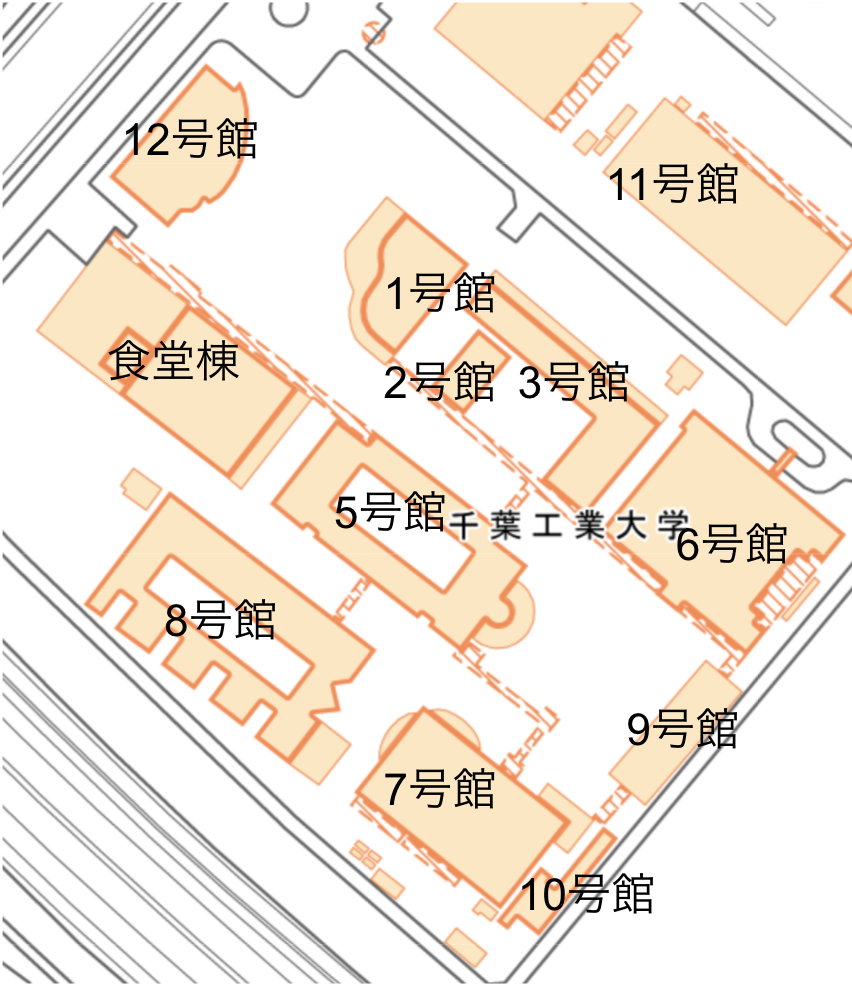
\includegraphics[height=6cm]{../images/metric_map.png}
             \label{subfigure::metric_map}}
             \subfigure[Map representing Chiba Institute of Technology Shin-Narashino Campus with topological map]{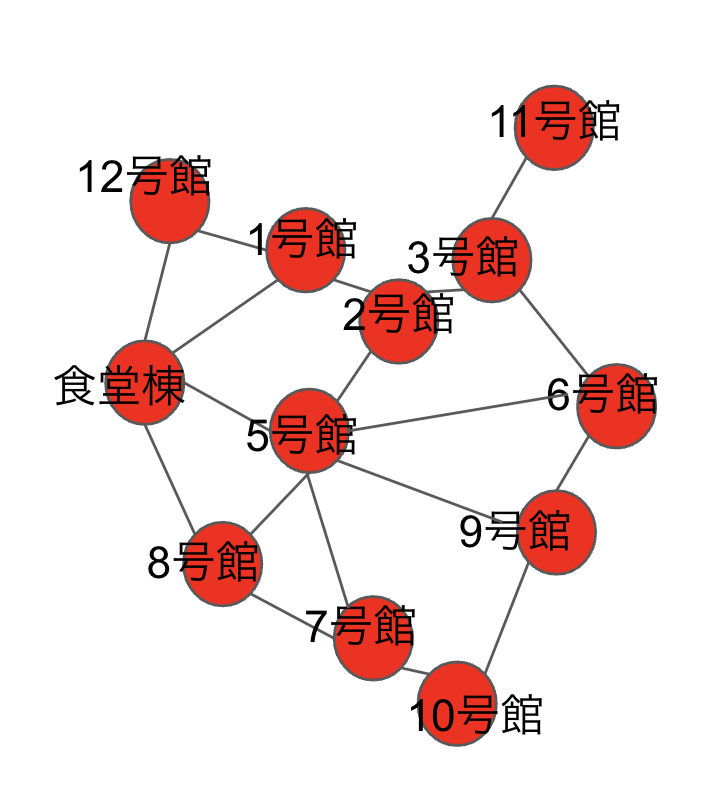
\includegraphics[height=6cm]{../images/topological_map.png}
             \label{subfigure::topological_map}}
             \caption{Example of metric and topological map}
             \label{figure::metric_and_topological_map}
          \end{figure}
          
        \newpage

        \section{シナリオ}
            シナリオとは,人間の道案内を文章で表現したものである.例えば,\fref{figure::scenario_exp}に表すような道案内の場合,シナリオは「次の角まで直進.右折.突き当たりまで直進.停止.」
            のようになる.また,シナリオは「次の角まで」や「突き当たりまで」のような条件と「直進」「右折」のような行動の組み合わせにより作成され,行動の後には「.」をつけて区切る必要がある.
        
        \begin{figure}[H]
         \centering
         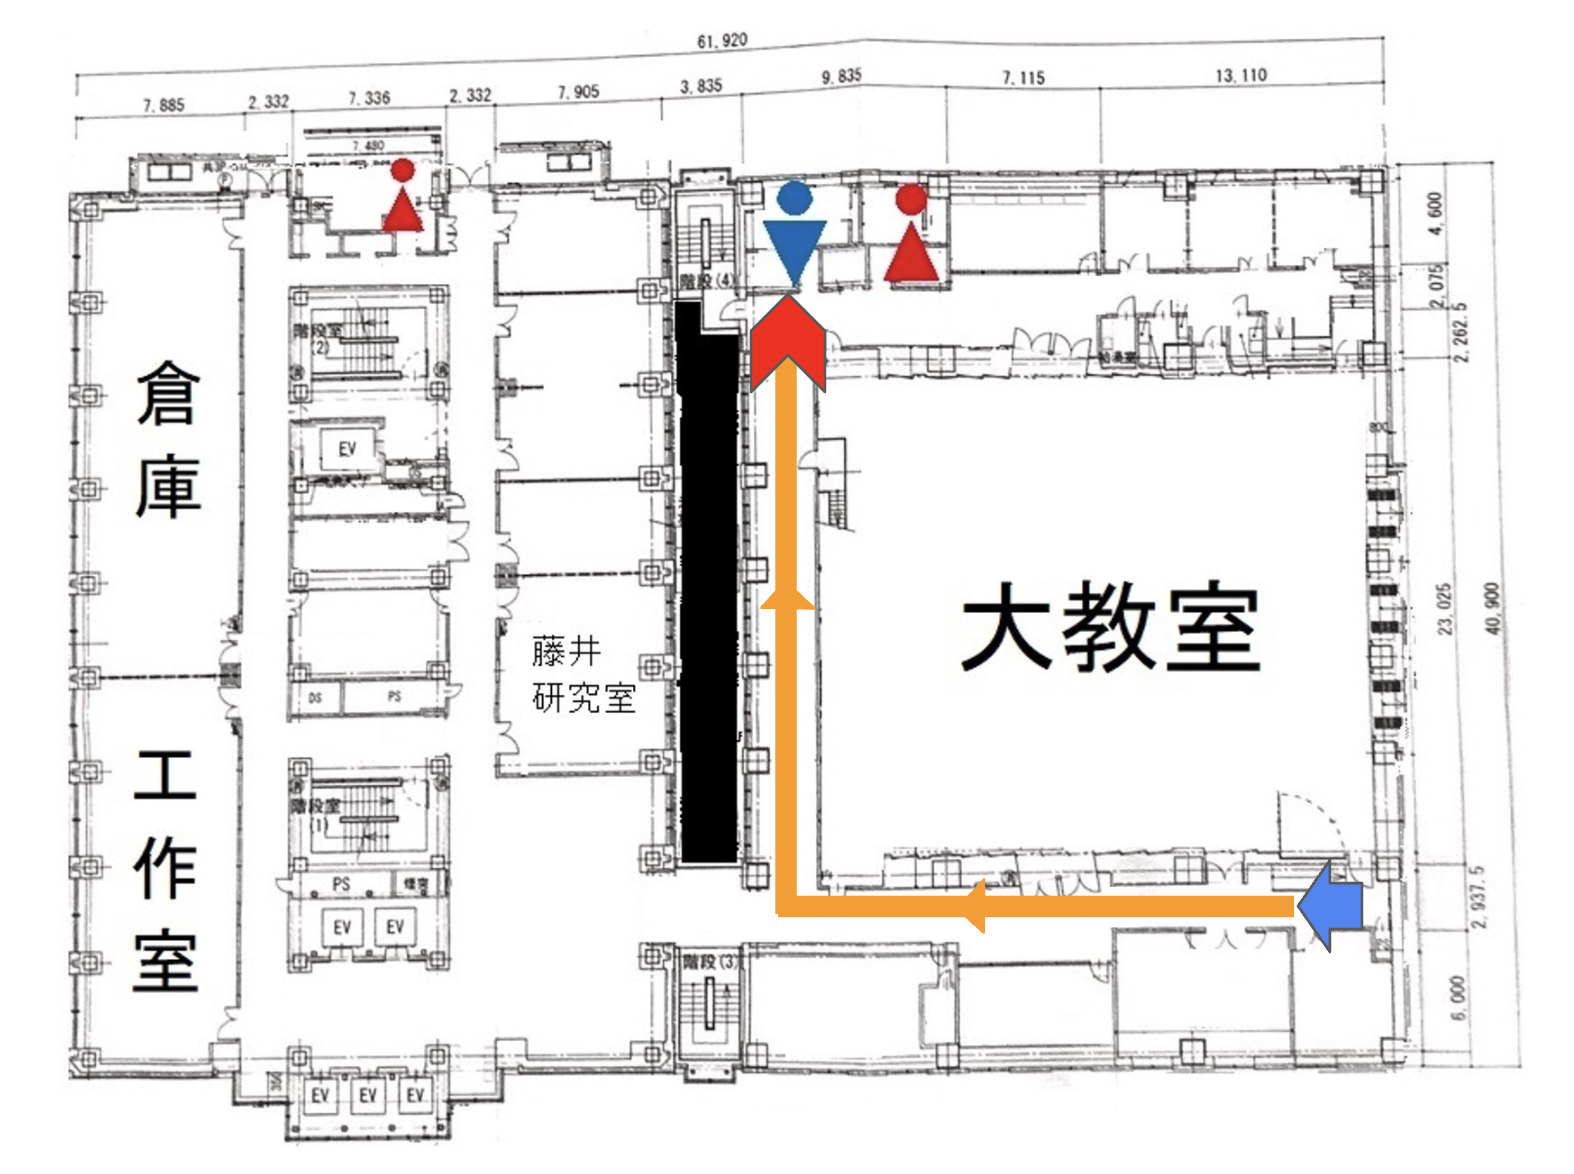
\includegraphics[width=12cm]{../images/scenario_fig}
         \caption{An example of human directions}
         \label{figure::scenario_exp}
        \end{figure}

        \newpage
          
        \section{Neural Network}
        ニューラルネットワークとは,人間の脳内の神経細胞(ニューロン)のネットワーク構造を模して作られた数式的なモデルである.
        ネットワークは,\fref{figure::NN}に示すように入力層,出力層,1つ以上の隠れ層(中間層)により構成されており,円で表されているものはニューロンと呼ぶ.
        また,線により結ばれているニューロンとニューロンの間には重みを持っており,重みは接続されているニューロン間のつながりの強さを表現している.
        ニューラルネットワークを用いることにより,複雑な回帰問題や分類問題などを解くことができる.
        \begin{figure}[H]
         \centering
         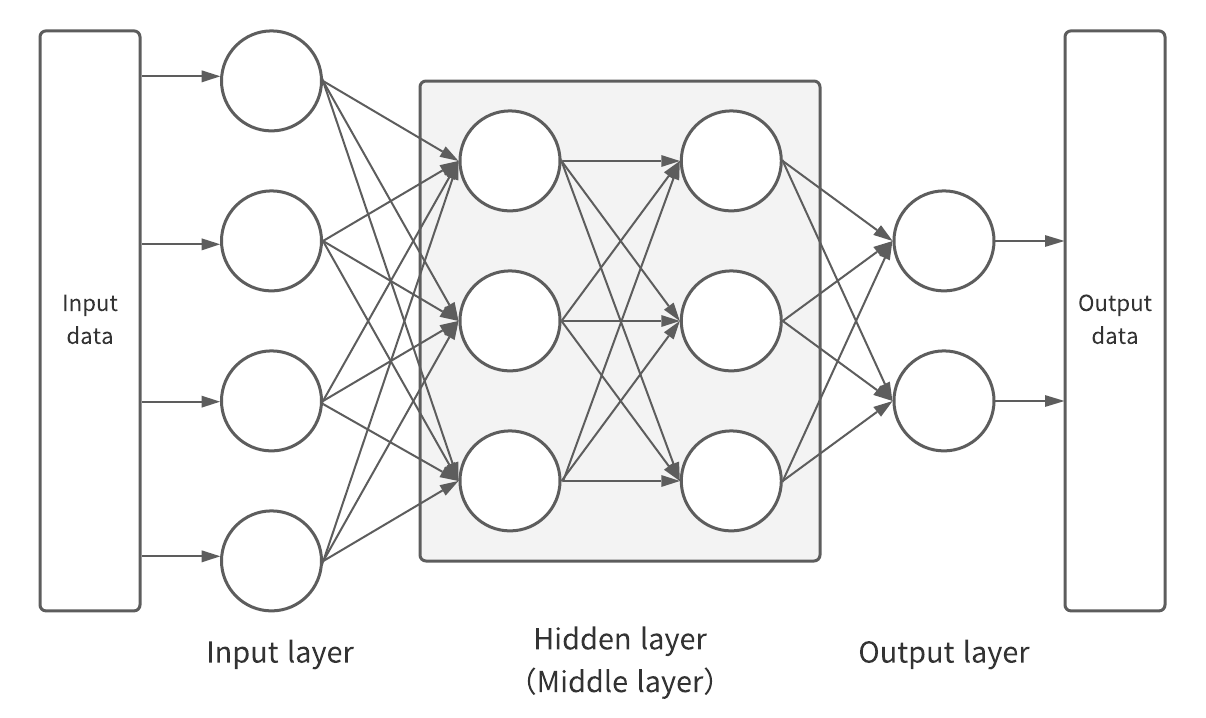
\includegraphics[width=12cm]{../images/NN.png}
         \caption{Neural network architecture}
         \label{figure::NN}
        \end{figure}

        \newpage
        
        \section{Convolutional Neural Network(CNN)}
        CNNはディープラーニングに手法の1つであり,ニューラルネットワークを元に作られている.
        ニューラルネットワークは入力層,中間層,出力層により構成されているが,
        CNNはニューラルネットワークの中間層に畳み込み層,プーリング層を組み込んだネットワークである.
        CNNにより画像認識をする場合の各層の役割を以下に記す.\\
        ・畳み込み層:入力した画像データにフィルタをかけ,特徴マップを出力することで特徴抽出を行う\\
        ・プーリング層:特徴マップをいくつかの領域に分割し,各領域で最大値または平均化を行うことで
        重要な情報を残しながら画像を縮小する.\\
        CNNは機械学習分野において主に画像・動画認識の分野で高い性能を発揮する.LeCunら\cite{cnn_paper}はCNNを用いて手書きの画像データから数字を識別できることを示し,その時のネットワークを
        \fref{figure::cnn}に表す.

        \begin{figure}[H]
         \centering
         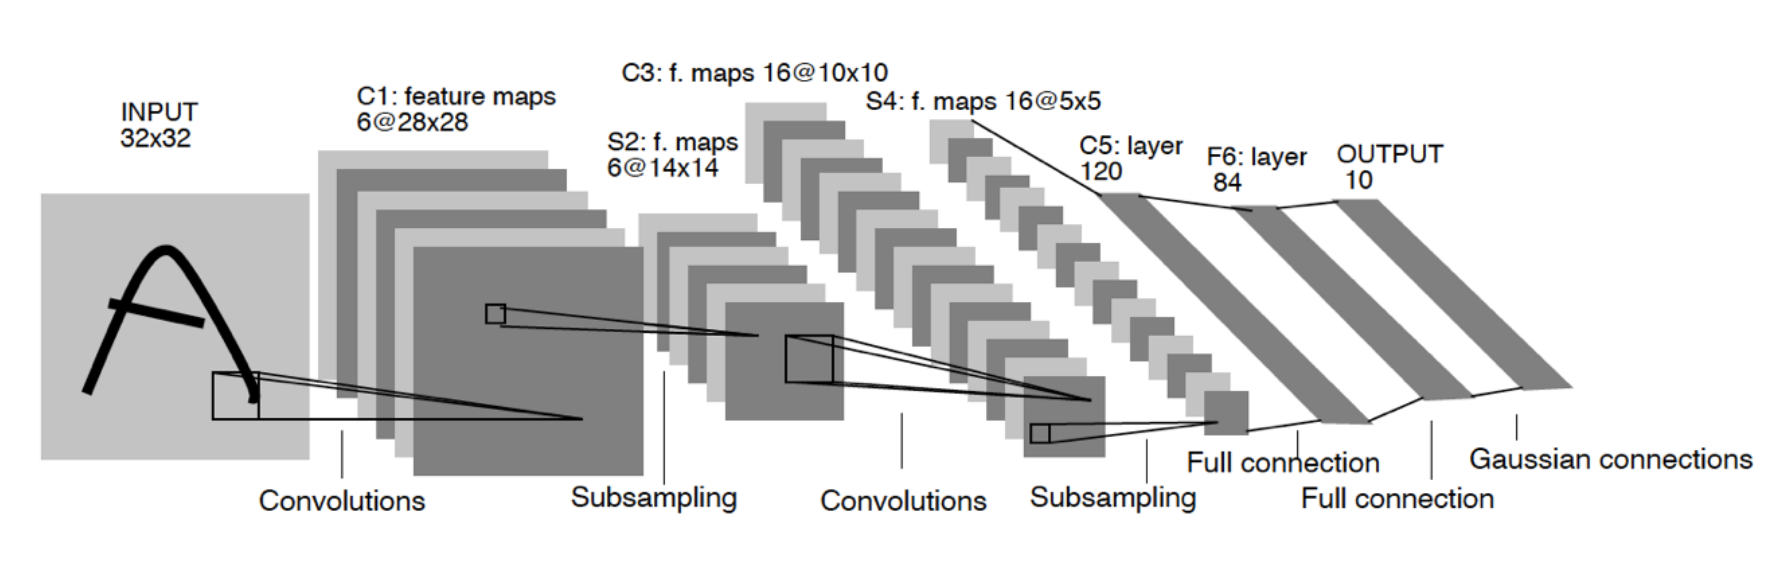
\includegraphics[width=15cm]{../images/cnn_exp.png}
         \caption{Architecture of CNN from\cite{cnn_paper}}
         \label{figure::cnn}
        \end{figure}

        \newpage

        \section{You Only Look Once(YOLO)}
        本研究で用いるYOLO\cite{yolo_paper_v1}\cite{yolo_paper_v2}\cite{yolo_paper_v3}\cite{yolo_paper_v4}は,リアルタイム物体検出アルゴリズムである.
        YOLOは,画像のRGBデータの配列をCNNに入力し,画像中のどの範囲に物体が存在しているのかを表すバウンディングボックスの情報と,
        ボックス内の物体がどのクラスに属しているのかを確率とともに表すクラス確率の情報を出力する.
        \fref{figure::yolo_exp}は,YOLOを用いて画像中の物体を検出している様子である. 

        \begin{figure}[H]
        \centering
        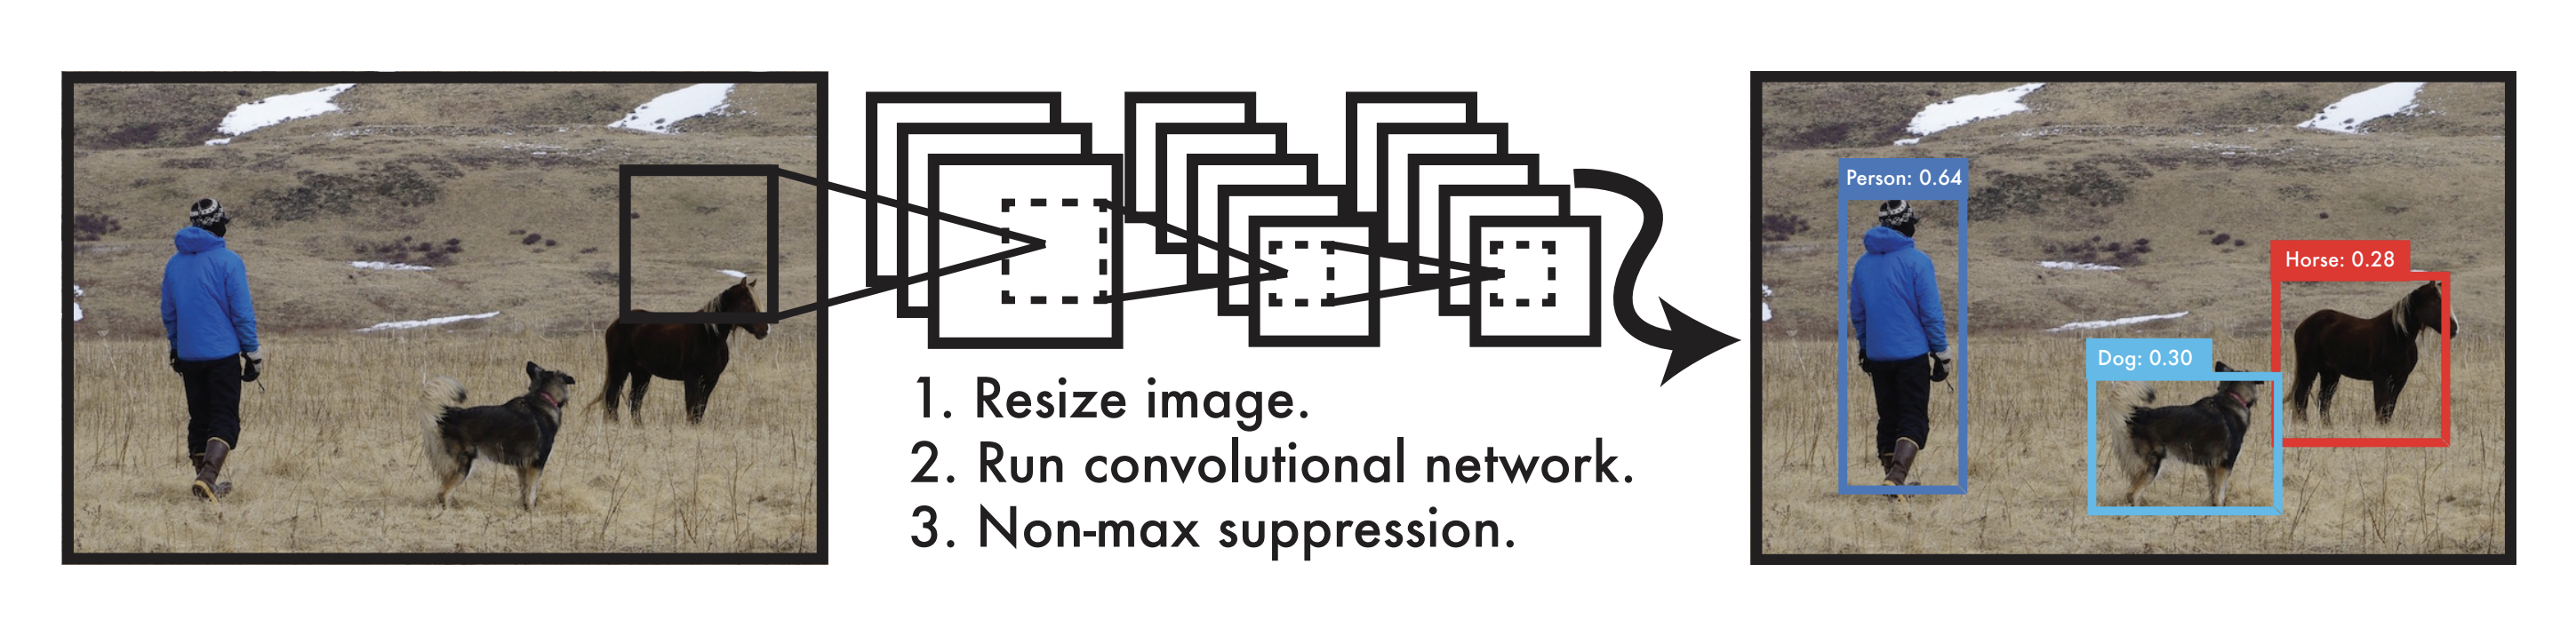
\includegraphics[width=10cm]{../images/yolo_exp.png}
        \caption{The YOLO Detection System.(出典:\cite{yolo_paper_v1})}
        \label{figure::yolo_exp}
        \end{figure}
        左の画像データを入力した結果,画像からは3つの物体が検出されている.
        また,それぞれの物体がPerson 0.64,Dog 0.30,Hose 0.28の確率で予測されていることが確認できる.
    \end{document}